\section{The Semantic Web Language Server}%
\label{sec:semantic_lsp}

This section is divided into two parts. The first outlines the key architectural design decisions, while the second details the implementation of each supported feature within this framework.

\subsection{Architecture design decisions}

The architectural design of the Semantic Web Language Server (SWLS) adheres to state-of-the-art implementation practices to ensure modularity, scalability, and maintainability~\cite{10.1145/3550355.3552452,10.1145/3563834.3567537,Bour_2018}, resulting in a \textit{Layered Architecture} containing three steps:

\begin{enumerate}
  \item In the \textit{Parse} step, the server handles parsing the document, which is language specific and deriving defined triples and prefixes.

  \item The \textit{Traverse} step derives information from the triples, such as defined properties, classes and SHACL shapes. 

  \item The \textit{Process} step is executed for each incoming request, extracting the required information from the previous steps and translates it into a response.
\end{enumerate}

SWLS is implemented in Rust and leverages Bevy’s Entity Component System (ECS)\footnote{\url{https://bevyengine.org/}} to adhere to the layered architecture.
An ECS is a software design pattern that organizes a program into four key elements: Entities, Components, Systems, and Resources. 
In SWLS, \textit{entities} represent the semantic documents. 
\textit{Components} store data associated with the entity, such as the document's contents, file location, or derived triples. 
\textit{Systems} are functions designed to process specific components, potentially adding other components to the entities.
\textit{Systems} are bundled into \textit{Schedules} to achieve distinct tasks.
\textit{Resources} are global components that are not linked to a specific entity.
For example, SWLS uses a resource to keep track of the hierarchy of discovered types, as types are not document specific.

% Bevy ECS facilitates this process by allowing the creation of isolated components and systems, enabling new features to be developed without impacting existing functionality.
% This modularity ensures that only the minimal required data is extracted for each task, avoiding the complexity and overhead of constructing a complete digital twin of the document at hand.
Together, these parts establish a structured framework in which implementing a new feature primarily involves integrating two new systems: one within the Traverse step to extract the necessary information and another within the Process step to enhance responses accordingly.
For instance, enabling autocompletion based on defined classes requires two additions: one mechanism to extract class definitions along with their descriptions and another to incorporate this information into autocompletion suggestions. 
This modular approach facilitates scalable and targeted development of language server functionalities.

As noted by Bour et al., ``No spec, no tests'' highlights the challenge of developing test suites for user-facing applications like language servers, where specifications can be open to interpretation~\cite{Bour_2018}. 
To address this, SWLS implements shared systems for common functionality, ensuring consistency and reducing redundancy across various Semantic Web languages.
By adopting this approach, SWLS delivers uniform features, while maintaining flexibility for language-specific extensions.

% SWLS is implemented in Rust and leverages Bevy’s Entity Component System (ECS)\footnote{\url{https://bevyengine.org/}} to maintain a highly modular and efficient architecture.
% Features are typically added in two steps:
%   first, extracting the necessary data from RDF triples and attaching it to relevant entities; 
%   second, using this data to implement language server functionalities such as diagnostics or autocompletion.

\subsection{Language Server schedules}

This section details the systems implemented within each schedule of SWLS.
Some systems are designed primarily to generate components, which are then utilized by other systems, potentially across different schedules.
This decoupled design ensures flexibility and modularity. 

\subsubsection{Parse}

\begin{figure}[tb]
 \centering
 \makebox[\textwidth]{%
    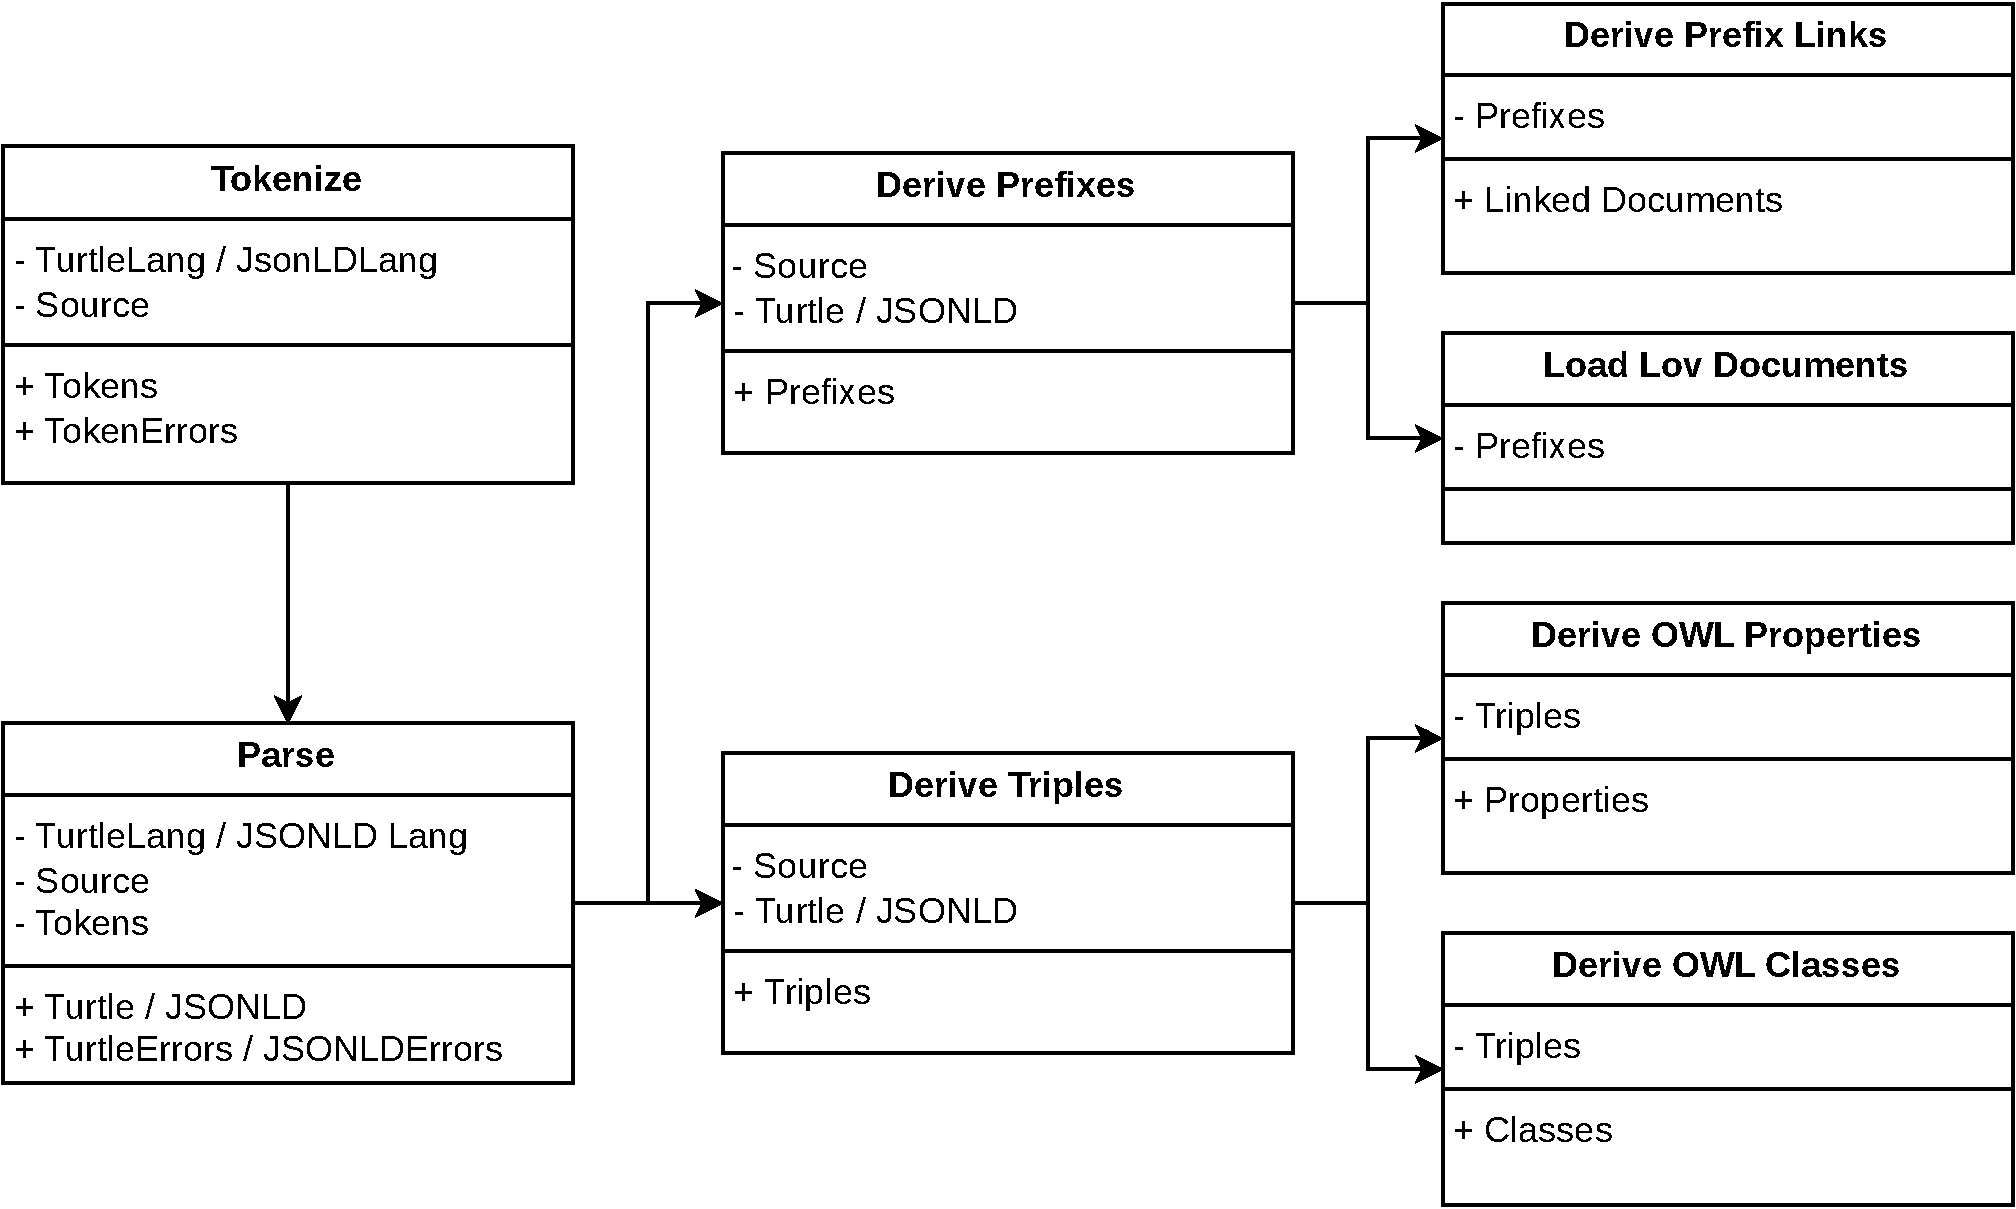
\includegraphics[width=1.2\textwidth]{./images/ParseSchedule.pdf}
 }
  \caption{Visual representation of the Parse schedule including tokenization, parsing, deriving prefixes, deriving triples, linking documents, fetching LOV documents, deriving properties and deriving classes. }\label{fig:Parse}
\end{figure}

The \textit{Parse} schedule is activated whenever the user edits a document, notifying the language server with the new contents, a visual overview is shown at Figure \ref{fig:Parse}.

First, \texttt{Tokenize} derives tokens from the incoming text document. SWLS uses the logos crate\footnote{\url{https://docs.rs/logos/latest/logos/}}. 
Each token corresponds to a terminal in the grammar. This system needs be implemented for each language.

The next system, \texttt{Parsing}, is implemented for each language and is responsible for transforming tokenized input into structured objects while reporting syntactic errors. 
SWLS employs Chumsky\footnote{\url{https://docs.rs/chumsky/latest/chumsky/}} to construct parser combinators for this purpose.
Significant effort has been invested in ensuring the parser can process faulty documents without discarding tokens: even isolated terms are expanded into full triples, facilitating downstream processing in subsequent stages.

However, expanding syntactically incorrect input introduces ambiguity.
For instance, the term \texttt{<a> <b> <c> <d>} could be expanded in multiple ways, such as: (i) \texttt{<a> <b> <c>. <d> <x> <y>.}, (ii) \texttt{<a> <b> <c>; <d> <x>.}, or (iii) \texttt{<a> <b> <c>, <d>}.
While the third option involves the fewest modifications, it does not always align with the expected behavior.
This ambiguity could be mitigated by leveraging partial parsing, which enables the parser to make more informed decisions based on incremental input changes.
However, this approach has not yet been implemented and remains an area for future work.

When the objects are parsed, language-specific systems derive prefixes and \textit{expanded} triples. 
Prefixes contain information about how to expand and shorten IRIs for the current document. 
After deriving triples, the next systems will derive properties and classes.
These properties and classes are later used to suggest autocompletions and derive type hierarchies.

SWLS introduces the concept of linked documents, documents that are related to the current document, which should be used for features like autocompletion.
Prefix statements are one way to link documents, but the object value of the triple \texttt{<> owl:imports <otherLocation>.}, also allows linking documents with the current document.
To acquire useful properties and classes, SWLS looks for ontology files, however we noticed that dereferencing the location of a prefix statement and expecting an ontology file is actually quite rare, 
so we introduced the LOV~\cite{LOV2017} service into SWLS.
Given a prefered prefix, SWLS will try to retrieve an ontology file and insert it into the language server, triggering the the parsing schedule for that document, which derives the actual properties and classes.

\subsubsection{Completion}

In the LSP, the server receives a completion event that contains the current cursor location of the user.
The server should then answer with a list of completions, including the textual operations, a title and potentially some documentation.

\begin{figure}[!ht]
 \centering
 \makebox[\textwidth]{%
    \includegraphics[width=1.2\textwidth]{./images/Completion.pdf}
 }
  \caption{Visual representation of the Completion schedule including GetCurrentToken, GetCurrentTriple, Subject Completion, Defined Prefix Completion, Prefix.cc Prefix Completion, Complete Classes and Complete Properties.}\label{fig:Completion}
\end{figure}

Figure~\ref{fig:Completion} shows a schematic overview of the different systems involved in the completion schedule and their interactions.
First the server will create a \texttt{CompletionRequest} object, containing no completions,
different systems then add their relevant completions to the request, which is then returned to the user.

The ECS has utility systems, like \texttt{GetCurrentToken} and \texttt{GetCurrentTriple} that map the current position to the current term and the current triple respectivily. This information is then added to the ECS entity. The current triple component also denotes which term of the triple is targeted (subject, predicate object or graph).

With the \texttt{CurrentToken} component, the server can suggest
\begin{itemize}
  \item Defined subjects with the \texttt{SubjectCompletion} system
  \item Defined prefixes in \texttt{Comlete Defined Prefix} system, this is language agnostic as the suggestions are derived from the \texttt{Prefix} component which is already generated.
  \item Importing new prefixes using prefix.cc\footnote{\url{https://prefix.cc}}, an online service that maps prefered prefixes to IRIs.
\end{itemize}

With the \texttt{CurrentTriple} component, SWLS suggests properties, if the user is writing a predicate.
SWLS tries to determine the type of the current subject, then SWLS orders properties in such a way that properties with the correct domain are shown first,
and visually distinguishes them from other properties.
When the user is typing an object and the predicate of the current triple is \texttt{rdf:type}, SWLS suggests defined classes.

\subsubsection{Diagnostics}

The \textit{Diagnostics} component of SWLS comprises several focused systems that analyze parsed data to identify issues and provide feedback to users.
Diagnostics differ from other language server functionalities as they are push-based: the server actively notifies the editor of errors and warnings.
This allows for timely feedback, ensuring that users can quickly identify and address problems in their documents.

Diagnostics are triggered with two schedules: \textit{on-edit} and \textit{on-save}.

\begin{enumerate}
  \item \textit{On edit} diagnostics provide fast, real-time feedback to users, enabling them to fix errors as they type. 
    This ensures a fluid editing experience and minimizes interruptions.
  \item \textit{On save} diagnostics occur less frequently and are therefore better suited to more computationally intensive checks,
   such as validation against SHACL shapes.
\end{enumerate}

To demonstrate the capabilities of the diagnostics system, we highlight three key systems:

\begin{enumerate}
  \item \textit{Syntax Diagnostics:}
    During the tokenization and parsing phases, errors such as syntax mismatches or malformed input are detected and recorded, along with their locations.
  \item \textit{SHACL Validation:} 
    With the on save schedule, the server uses the Rudof library\footnote{\url{https://github.com/rudof-project/rudof}} to validate the current RDF document against SHACL and ShEx shapes~\cite{labra2022rudof}.
    Shapes are extracted from the document itself (if present), as well as other linked documents.
    This system ensures that the semantic data conforms to expected structural constraints, enabling robust validation.
  \item \textit{Basic Validation:}
    This system identifies common issues, such as undefined prefixes or unused declarations.
    By flagging such problems, users can better maintain consistency and avoid errors that might lead to interoperability issues.
\end{enumerate}

Together, these systems provide comprehensive diagnostic support, catering to both immediate feedback needs and more in-depth validation processes.

\subsubsection{Others}

Beyond core functionalities, SWLS offers additional schedules that enhance the user experience and round out its capabilities.
These schedules are smaller in scope, generally focusing on presentation or user interaction rather than deriving new information.

The most notable are the following:
\begin{enumerate}
  \item \textit{Formatting:}
    A consistent document structure improves readability and reduces the cognitive load required to parse data visually.
    As a formatter, the language server ensures uniformity across documents, promoting best practices and easing collaboration.
    Currently, the SWLS includes an opinionated formatter for Turtle.

  \item \textit{Hover:}
    Hover functionality provides contextual insights about symbols in the document, offering users additional information without disrupting their workflow,
    allowing for users to explore semantic relationships and documentation seamlessly.
    The SWLS’s hover implementation includes three key features:
    \begin{itemize}
      \item Type Information: For a node with an inferred type, the hover popup displays the type alongside its hierarchy, including subclasses and superclasses.
      \item Class Details: Hovering over a class reveals its \texttt{rdfs:description}.
      \item Property Insights: Hovering over a property shows its \texttt{rdfs:description}, as well as its range and domain.
    \end{itemize}

  \item \textit{Highlighting:}
    Highlighting improves document readability by visually distinguishing between elements.
    The SWLS implements both syntax highlighting and semantic highlighting through a two-step process:
        (i) An initial system maps all tokens to their basic semantic types.
        (ii) Subsequent systems refine the types based on additional information.
    For example, in JSON-LD, all keys are initially highlighted as strings.
    However, keys starting with the \texttt{@} symbol are reclassified as keywords, enhancing clarity and usability for JSON-LD documents.
\end{enumerate}

These schedules, while smaller in scale, enhance the language server’s utility by making semantic documents more intuitive and easier to work with.
They represent the \textit{polish} that transforms SWLS into a complete tool for Semantic Web practitioners.